
%%%%%%%%%%%%%%%%%%%%%%%%%%%%%%%%%%%%%%%%%%%%%%%%%
%%%%%%%%%%%%%%%%%%%%%%%%%%%%%%%%%%%%%%%%%%%%%%%%%
%%%%%%%%%%%%%%%%%%%%%%%%%%%%%%%%%%%%%%%%%%%%%%%%%

\section[Обзор метрик]{Обзор метрик семантической близости} 
\subsection{  }


\begin{frame}
\frametitle{Обзор метрик семантической близости}

\textbf{Публикации} 
\begin{itemize}
\item Panchenko A., \textbf{Similarity Measures for Semantic Relation Extraction.} PhD thesis. Universit\'{e} catholique de Louvain. 197
pages, 2013: \alert{Chapters 2.1, 3.1}. 
\item Panchenko A. \textbf{A Study of Heterogeneous Similarity Measures for Semantic Relation Extraction.} // In JEP-TALN-RECITAL 2012 — Grenoble (France), 2012.

\item ACL Anthology / Google Scholar: \alert{``semantic similarity measure''}, \alert{``semantic similarity''}. 
\end{itemize}
 
\end{frame}



\begin{frame}
\frametitle{Обзор метрик семантической близости}

\begin{figure}
\includegraphics[width=1.05\textwidth]{./../figures/measures-classification}
\end{figure}

\textbf{Публикации} (анализ 37 базовых метрик):
\begin{itemize}
\item Panchenko A., \textbf{Similarity Measures for Semantic Relation Extraction.} PhD thesis. Universit\'{e} catholique de Louvain. 197
pages, 2013, (Chapter 3). 
\item Panchenko A. \textbf{A Study of Heterogeneous Similarity Measures for Semantic Relation Extraction.} // In JEP-TALN-RECITAL 2012 — Grenoble (France), 2012. 
\end{itemize}
 
\end{frame}



%%%%%%%%%%%%%%%%%%%%%%%%%%%%%%%%%%%%%%%%%%%%%%%%%
\begin{frame}
\frametitle{Метрики, основанные на семантической сети}

 \textbf{Данные:} семантическая сеть WordNet 3.0, корпус SemCor.
    
 \textbf{Переменные:}
\begin{itemize}
\item $len(c_i,c_j)$ -- длина \textbf{кратчайшего пути} между $c_i$ и $c_j$
\item  $len(c_i, lcs(c_i,c_j))$ -- длина кратчайшего пути от $c_i$ до \textbf{ближайшего общего предка  (БОП)} слов $c_i$ и $c_j$

\item Ближайший Общий Предок (БОП) -- Lowest Common Subsumers (LCS) 

\item $len(c_{root}, lcs(c_i,c_j))$ -- длина кратчайшего пути от \textbf{корня} $c_{root}$ до БОП слов $c_i$ и $c_j$ (глубина БОП)
\item $P(c)$ --  \textbf{вероятность слова} $c$, оцененная из корпуса
\item  $P(lcs(c_i, c_j))$ -- \textbf{вероятность БОП} слов $c_i$ и $c_j$
\end{itemize}
    
    
\textbf{Метрики:} Инвертированная длина пути, Leacock-Chodorow, Wu-Palmer, 
 Resnik, Jiang-Conrath, Lin.
  
\end{frame}




\begin{frame}
\frametitle{Lowest common subsumer (LCS) }

\begin{figure}
\centering
\includegraphics[width=0.55\textwidth]{../figures/lcs-example}
\caption{Ближайшие общие предки в семантической сети.}
\end{figure}
    
\begin{itemize}
  \item $(car, food) \rightarrow object$
  \item $(beef, pork) \rightarrow meat$
  \item $(pork, coupe) \rightarrow object$
  \item $(vegetable, pork) \rightarrow food$
\end{itemize}

\end{frame}






\begin{frame}
\frametitle{Метрики, основанные на семантической сети}

\begin{itemize}

\item \textbf{Инвертированная длина пути}:

$$
s_{ij}=len(c_i,c_j)^{-1}.
$$

\item \textbf{LeacockChodorow}: 
$$
s_{ij}=-\log\frac{len(c_i,c_j)}{2h}.
$$

\item \textbf{Resnik}: 
$$
s_{ij}=-\log P(c_{ij}).
$$ 


\item \textbf{JiangConrath}: 
$$
d_{ij}= 2 \log P(c_{ij}) - (\log P(c_i) + \log P(c_j)).
$$

\end{itemize}

\end{frame}






\begin{frame}
\frametitle{Метрики, основанные на семантической сети}


\begin{itemize}

\item \textbf{Lin}: $$ s_{ij}= \frac{2 \log(P(c_{ij}))}{\log(P(c_i) + \log(P(c_j))  } $$

\item \textbf{WuPalmer}: 
$$ s_{ij}=\frac{2  len(c_{r},c_{ij})}{len(c_i,c_{ij})+len(c_j,c_{ij})+2\cdot len(c_{r},c_{ij})} $$
 
\end{itemize}
\end{frame}






\begin{frame}
\frametitle{Метрики, основанные на семантической сети}

\textbf{Инструменты}:

\begin{itemize}
\item WordNet::Similarity tool (Perl, command-line): \url{http://wn-similarity.sourceforge.net/}

\item NTLK (Python): \url{http://nltk.org}

\end{itemize}

\begin{figure}
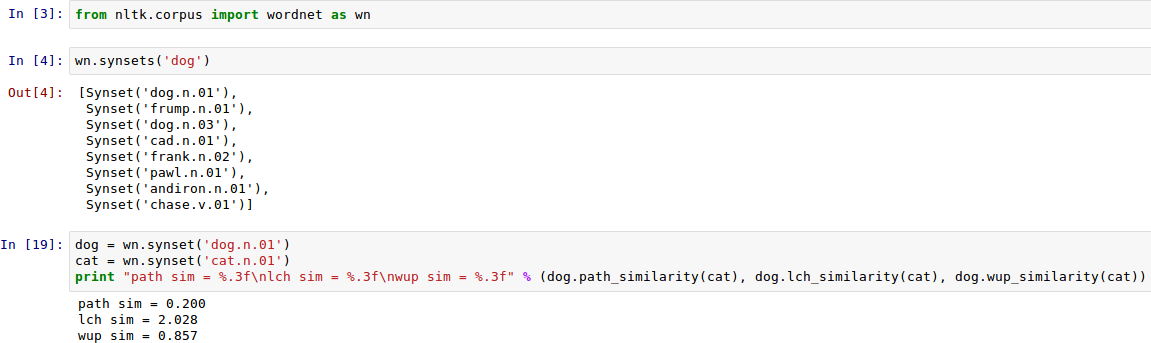
\includegraphics[width=1.0\textwidth]{./figures/python-example}
\end{figure}

\tiny{
Источник: \url{http://googlecode.com/svn-/trunk/doc/howto/wordnet.html}
}


\end{frame}







%%%%%%%%%%%%%%%%%%%%%%%%%%%%%%%%%%%%%%%%%%%%%%%%%
\begin{frame}
\frametitle{Метрики, основанные на Веб корпусе текстов }

\textbf{Данные:} количество документов возвращенных ИПС: Google, 
Yahoo, AltaVista, Bing, и т.п.
    
\textbf{Переменные:} 
\begin{itemize}
    \item $h_i$ -- \textbf{количество документов} возвращенных по запросу слова
    $"c_i"$
    \item $h_{ij}$ -- \textbf{количество документов} возвращенных по запросу $"c_i \text{ AND } c_j"$
\end{itemize}

\textbf{Метрики:} 
\begin{itemize}
\item Normalized Google Distance (NGD) (Cilibrasi and Vitanyi, 2007)
\item Pointwise Mutual Information - Information Retrieval (PMI-IR) (Turney,
2001)
\end{itemize}
\end{frame}








%%%%%%%%%%%%%%%%%%%%%%%%%%%%%%%%%%%%%%%%%%%%%%%%%
\begin{frame}
\frametitle{ Веб-метрики: пример }

 \begin{figure}
  \centering
   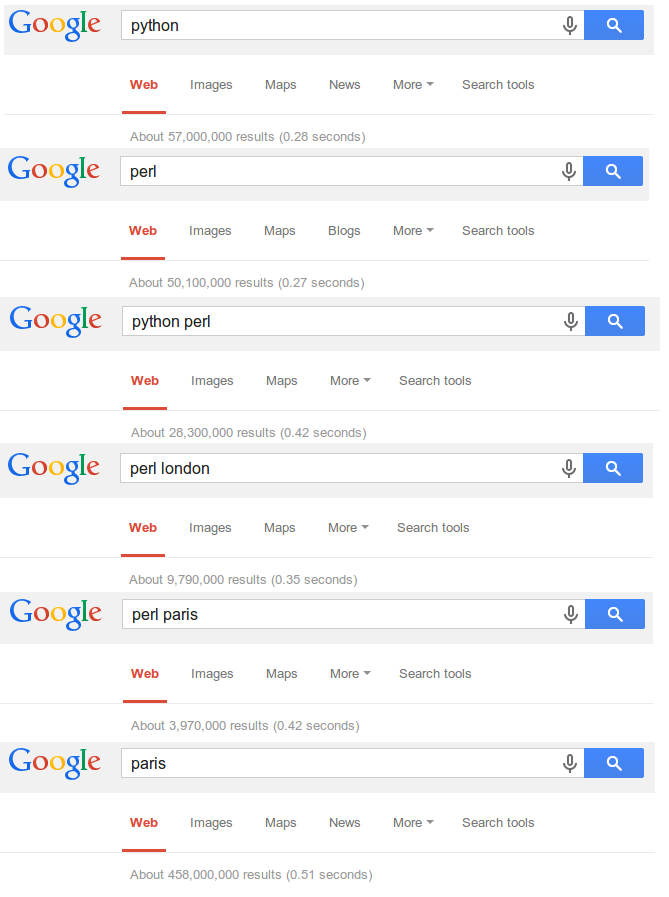
\includegraphics[width=0.5\textwidth]{./figures/google-web}
 \end{figure}

\end{frame}







\begin{frame}
\frametitle{Метрики, основанные на Веб корпусе текстов }

\begin{itemize}
\item \textbf{Normalized Google Distance (NGD)}: 
 
 $$ s_{ij}=\frac{max(log(h_i), log(h_j))-log(h_{ij})}{log(M)-min(log(h_i),log(h_j))} $$

\item \textbf{Pointwise Mutual Information Information Retrieval (PMIIR)}:
$$
s_{ij}= \log \frac{P(c_i,c_j)}{P(c_i) P(c_j)} = \log \frac{ \frac{h_{ij}}{\sum_{i,j} h_{ij}} }{ \frac{h_{i}}{\sum_{i,j} h_{ij}} \frac{h_{j}}{\sum_{i,j} h_{ij}} } \approx \log \frac{h_{ij} }{h_i h_j} .
$$

\end{itemize}

\end{frame}








%%%%%%%%%%%%%%%%%%%%%%%%%%%%%%%%%%%%%%%%%%%%%%%%%
\begin{frame}
\frametitle{Дистрибутивные метрики}

\textbf{Данные:} корпус, такой как Википедия или ukWaC

\begin{figure}
\centering
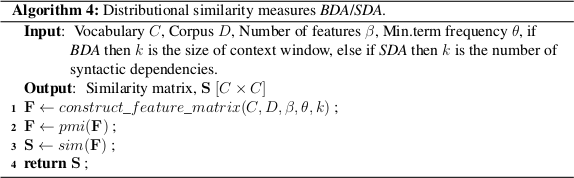
\includegraphics[width=0.8\textwidth]{./figures/dist-sem-algo}
\end{figure}

\textbf{Метрики:}
\begin{itemize}
    \item Bag-of-words Distributional Analysis (BDA) (Sahlgren, 2006)
    \item Syntactic Distributional Analysis (SDA) (Curran, 2003)
\end{itemize}
    
\end{frame} 
    
    
    
\begin{frame}
\frametitle{Дистрибутивные метрики}

\textbf{Переменные:} 
\begin{itemize}

\item $\textbf{f}_i$-- вектор признаков представляющий слово $c_i$, основанный на \textbf{контекстном окне}

\item $ \mathbf{f}^s_i$ -- вектор признаков представляющий слово $c_i$, основанный на \textbf{синтаксическом контекстном окне}
\begin{figure}
\includegraphics[width=0.9\textwidth]{./../figures/10-figure-3-gray}
\end{figure}

\begin{figure}
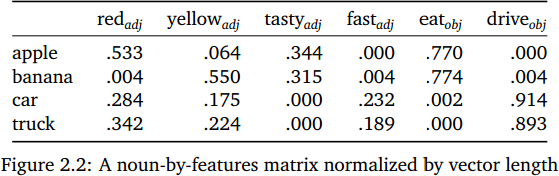
\includegraphics[width=0.6\textwidth]{./figures/sda-table}
\end{figure}

\tiny{\textbf{Источник}: Tim Van de Cruys, Mining for Meaning, PhD thesis (2010)}

   
\end{itemize}
    
    
\end{frame}
    




\begin{frame}
\frametitle{Другие метрики, основанные на корпусе текстов}

\textbf{Данные:} корпус, такой как Википедия или ukWaC
    
    
\textbf{Метрики:}
\begin{itemize} 
\item Латентно-cемантический анализ (LSA) (Landauer and Dumais, 1997)
\item Вероятностные модели (pLSA, LDA и др.) (Griffiths et al., 2007)
\item NGD и PMI-IR (Veksler et al., 2008)
\item \ldots
\end{itemize}
    
\end{frame}



\begin{frame}
\frametitle{Латентно-семантический анализ}
\textbf{Latent Semantic Analysis (LSA)} (Landauer and Dumais, 1997):

\begin{enumerate}
\item Representing the corpus $D$ as an $N \times M$ term-document matrix $\mathbf{F}$.

% An element $f_{ij} \in \mathbf{F}$ of this matrix contains frequency of the word $w_i$ in the document $d_j \in D$. 

\item  Normalization of the matrix $\mathbf{F}$ with TF-IDF:
$$
f_{ij}^\prime = \frac{f_{ij}}{\sum_i f_{ij}} \cdot log \frac{|D|}{|d \in D : w_i \in d|},
$$


\item Singular value decomposition of $\mathbf{D}$: $ \mathbf{D} = \mathbf{U} \Sigma \mathbf{V}^T.$

\item Low-rank approximation of the matrix $\mathbf{U}$ with a reduced $M \times k$ matrix $\mathbf{U}_k$ by retaining only the first $k$ column of the $\mathbf{U}$. 

\item Calculation of similarities between terms $c_i$ and $c_j$ as a cosine between respective columns of $\mathbf{U}_k$ ($\mathbf{u}^k_i$ and $\mathbf{u}^k_i$):

$$
s_{ij} = \frac{\mathbf{u}^k_i \cdot \mathbf{u}^k_j}{||\mathbf{u}^k_i|| ||\mathbf{u}^k_j ||}.
$$

\end{enumerate}

\end{frame}







\begin{frame}
\frametitle{Латентно-семантический анализ}

\begin{itemize}

\item $\mathbf{U}$ is an $M \times M$ matrix which columns are the orthogonal eigenvectors of $\mathbf{D D}^T$
\item  $\mathbf{V}^T$ is an $N \times N$ matrix which columns are the orthogonal eigenvectors of $\mathbf{D}^T \mathbf{D}$

\item $\Sigma$ is an $M \times N$ diagonal matrix:

$$
\Sigma = \begin{pmatrix}
  \sigma_{11} & \ldots & 0 \\
  \vdots  & \ddots & \vdots  \\
  0 & \cdots & \sigma_{nn}
 \end{pmatrix}.
$$

\item The $i$-th element on the diagonal $\sigma_{ii} = \sqrt{\lambda_i}$, where $\lambda_i$ is an eigenvalue of $\mathbf{D D}^T$. 

\item The eigenvalues are ordered, such that $\lambda_i \geq \lambda_{i+1}$.  

\end{itemize}

\tiny{\textbf{Источник}: Manning et al. Introduction to information retrieval (2008), p.374.}

\end{frame}




\begin{frame}
\frametitle{Латентно-семантический анализ}

\begin{figure}
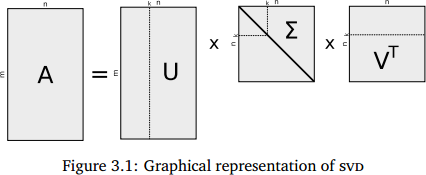
\includegraphics[width=0.8\textwidth]{./figures/lsa}
\end{figure}

\tiny{\textbf{Источник}: Tim Van de Cruys, Mining for Meaning, PhD thesis (2010)}

\end{frame}




%%%%%%%%%%%%%%%%%%%%%%%%%%%%%%%%%%%%%%%%%%%%%%%%%
\begin{frame}
\frametitle{Метрики, основанные на определениях}

\textbf{Данные:} определения из WordNet, Википедии, Викисловаря или любого
другого словаря.
    
\textbf{Переменные:}
\begin{itemize}
        \item $gloss(c_i)$ -- \textbf{определение} слова $c_i$;
        \item $\mathbf{f}_i$ \textbf{вектор признаков}, построенный из $gloss(c_i)$;
        \item $\mathbf{f}_i$ -- \textbf{вектор признаков} $c_i$, вычисленный на
        корпусе из всех определений методом контекстного окна;
        
        \item $exist(c_i, c_j)$ -- наличие связи между $c_i$ и $c_j$ в словаре.
\end{itemize}

\textbf{Метрики:}
\begin{itemize}
  \item ExtendedLesk (Banerjee and Pedersen, 2003)
  \item GlossVectors (Patwardhan and Pedersen, 2006)
  \item DefVectors (Panchenko et al., 2012)
  
\end{itemize}

\end{frame}





\begin{frame}
\frametitle{Метрики, основанные на определениях: Extended Lesk}

\begin{itemize}
\item relies on the gloss similarity of terms $c_i$ and $c_j$
\item relies on gloss similarity of all terms related to $c_i$ and $c_j$  

$$
s_{ij}=\sum_{c_i \in C_i}\sum_{c_j \in C_j} sim_g(c_i,c_j),
$$
\item $sim_g$ is a gloss-based similarity measure and set $C_i$ includes concept $c_i$ and all concepts directly related to it. 
\end{itemize}

\end{frame}


\begin{frame}
\frametitle{Метрики, основанные на определениях: GlossVectors}


\begin{itemize}
\item a cosine between vectors $\mathbf{v}_i$ and $\mathbf{v}_j$ representing concepts $c_i$ and $c_j$

\item a vector $\mathbf{v}_i$ is a sum of context vectors representing all words from the definition of $c_i$ and the definitions of terms related to $c_i$:

$$
s_{ij} =  \frac{\mathbf{v}_i \cdot \mathbf{v}_j}{||\mathbf{v}_i|| ||\mathbf{v}_j||} \text{ where } \mathbf{v}_i = \sum_{ \forall j : c_j \in G_i  } \mathbf{f}_j.
$$

\item $\mathbf{f}_j$ is a context vector, derived from the corpus of all glosses 
\item $G_i$ is concatenation of glosses of the concept $c_i$ and all concepts which are directly related to it.

\end{itemize}

\end{frame}





\begin{frame}
\frametitle{Сравнение базовых метрик семантической близости}



\begin{figure}
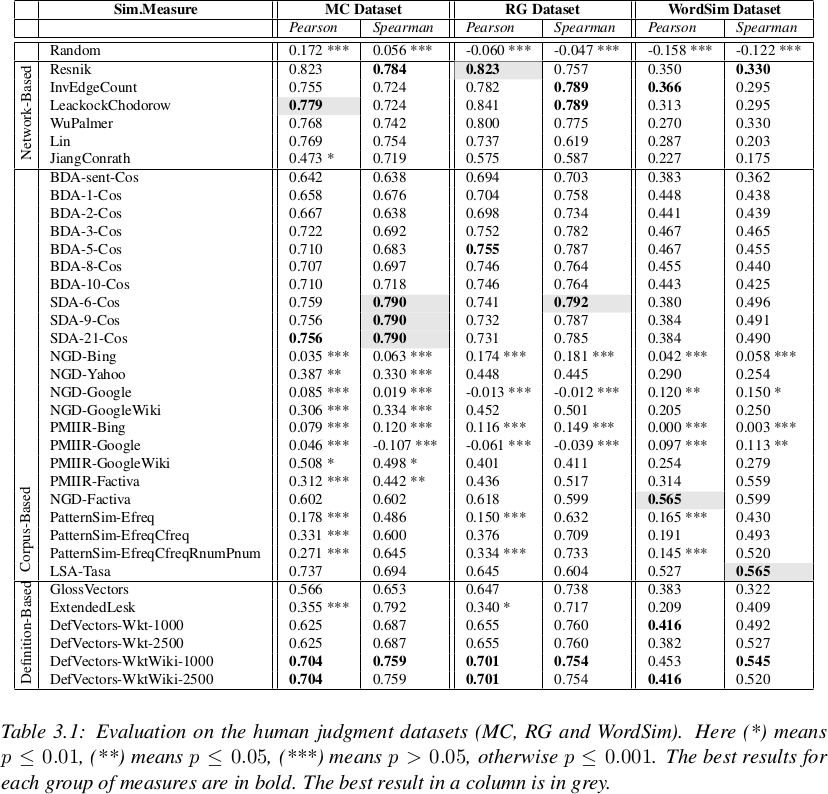
\includegraphics[width=0.69\textwidth]{./figures/overview-table1}
\end{figure}
   
\end{frame}





\begin{frame}
\frametitle{Сравнение базовых метрик семантической близости}

\begin{figure}
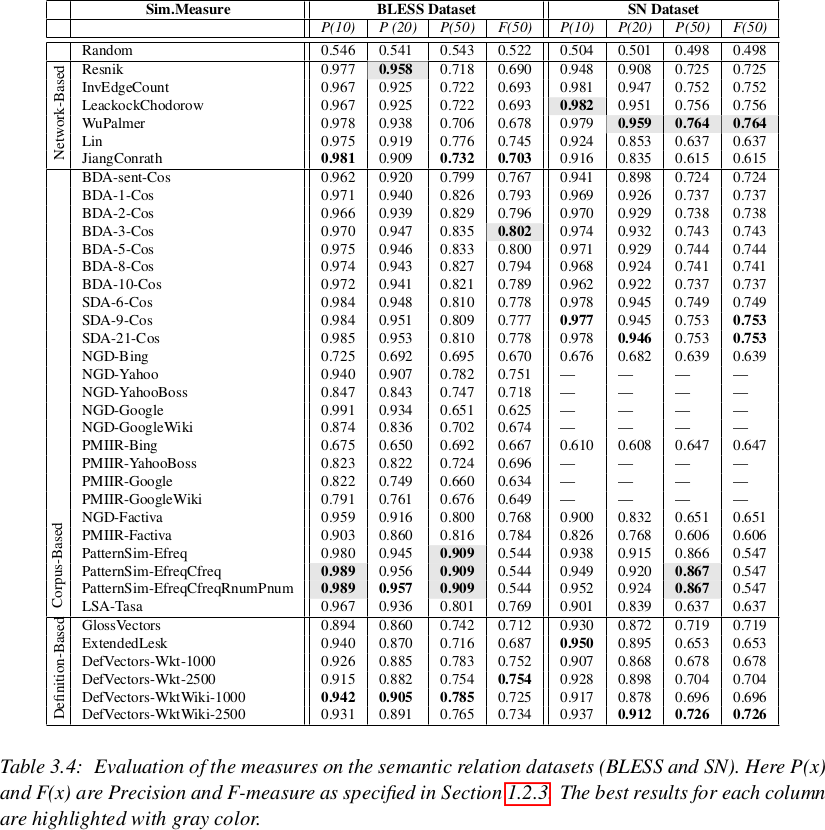
\includegraphics[width=0.65\textwidth]{./figures/overview-table2}
\end{figure}
   
\end{frame}






\begin{frame}
\frametitle{Сравнение: лучшие базовые метрики}

\begin{figure}
\includegraphics[width=1.05\textwidth]{./../figures/best}

\end{figure}

\begin{itemize}
  \item Каждая метрика излекает много \alert{ко-гипонимов}: 
  \begin{itemize}
  \item $\langle Canon, Nikon \rangle$,
  \item $\langle Lamborghini, Ferrari \rangle$,
  \item $\langle Obama, Romney \rangle$.
\end{itemize}
\end{itemize}
   
\end{frame}





\begin{frame}
\frametitle{Резюме}

\begin{block}{Основные ресурсы для построения метрик:}
\begin{itemize}
  \item семантические сети и тезаурусы;
  \item корпуса текстов;
  \item Веб корпус текстов;
  \item определения из словарей и энциклопедий. 
\end{itemize}
\end{block}   


\begin{block}{Метрики \textbf{дополняют друг друга} в терминах:}
\begin{itemize}
  \item лексического покрытия;
  \item точности;
  \item типов извлекаемых отношений. 
\end{itemize}
\end{block}   

\end{frame}





\begin{frame}
\frametitle{Программное обеспечение}

\begin{itemize}
  \item \textbf{Semantic Vectors:} \url{https://code.google.com/p/semanticvectors/}
  \item \textbf{S-Space Package:} \url{https://code.google.com/p/airhead-research/}
  \item \textbf{WordNet::Similarity:} \url{http://wn-similarity.sourceforge.net}
  \item \textbf{NLTK:} \url{http://nltk.googlecode.com/svn/trunk/doc/howto/wordnet.html}
  \item \textbf{WikiRelate!}
  \item \textbf{PatternSim / Serelex:} \url{http://serelex.cental.be}
  \item \textbf{Метрики, основанные на Веб корпусе:} \url{http://cwl-projects.cogsci.rpi.edu/msr}
  \item \textbf{LSA:} \url{http://lsa.colorado.edu}
  \item \textbf{DefVectors:} \url{http://github.com/jgc128/defvectors}
\end{itemize}

\end{frame}
